\documentclass[aspectratio=169]{beamer}

% ---------- Theme & Color ----------
\usetheme{Madrid}
\usecolortheme{default}

\definecolor{sctceblue}{RGB}{0, 51, 102}
\definecolor{accentblue}{RGB}{0, 102, 204}
\definecolor{lightgray}{RGB}{240, 240, 240}
\definecolor{darkgray}{RGB}{60, 60, 60}

\setbeamercolor{palette primary}{bg=sctceblue, fg=white}
\setbeamercolor{palette secondary}{bg=accentblue, fg=white}
\setbeamercolor{palette tertiary}{bg=sctceblue!80, fg=white}
\setbeamercolor{palette quaternary}{bg=sctceblue, fg=white}
\setbeamercolor{structure}{fg=sctceblue}
\setbeamercolor{section in toc}{fg=sctceblue}
\setbeamercolor{frametitle}{bg=sctceblue, fg=white}
\setbeamercolor{title}{fg=white}
\setbeamercolor{block title}{bg=accentblue, fg=white}
\setbeamercolor{block body}{bg=lightgray, fg=darkgray}
\setbeamercolor{alerted text}{fg=accentblue}

% ---------- Fonts ----------
\usepackage{lmodern}
\usepackage[T1]{fontenc}
\usepackage[utf8]{inputenc}

% ---------- Packages ----------
\usepackage{booktabs}
\usepackage{array}
\usepackage{tabularx}
\usepackage{graphicx}
\usepackage{tikz}
\usetikzlibrary{shapes.geometric, arrows.meta, positioning, fit, backgrounds}
\usepackage{amsmath}
\usepackage{xcolor}
\usepackage{multirow}
\usepackage{fontawesome5}

% ---------- Image Path ----------
% Keep architecture.jpg, workflow.jpg, and cart.jpg in the same folder as this .tex file.
\graphicspath{{./}}

% ---------- Footer ----------
\setbeamertemplate{footline}{
  \leavevmode
  \hbox{%
    \begin{beamercolorbox}[wd=.33\paperwidth,ht=2.25ex,dp=1ex,center]{palette primary}%
      \usebeamerfont{author in head/foot}\insertshortauthor
    \end{beamercolorbox}%
    \begin{beamercolorbox}[wd=.34\paperwidth,ht=2.25ex,dp=1ex,center]{palette secondary}%
      \usebeamerfont{title in head/foot}\insertshorttitle
    \end{beamercolorbox}%
    \begin{beamercolorbox}[wd=.33\paperwidth,ht=2.25ex,dp=1ex,right]{palette tertiary}%
      \usebeamerfont{date in head/foot}\insertframenumber{} / \inserttotalframenumber\hspace*{2ex}
    \end{beamercolorbox}}
}
\setbeamertemplate{navigation symbols}{}

% ---------- Title Info ----------
\title[AutoMatch]{AutoMatch -- Intelligent Vehicle Recommendation System}
\subtitle{Mini Project -- CMD334}
\author[Aadil | Adithyan | Adhway]{%
  Aadil Sandeep (301) \and Adithyan R (305) \and Adhway Satheesh (366)\\[0.4em]
  \small Guided By: \textbf{Dr.\ Rejimoan R}
}
\institute[SCTCE]{%
  B.Tech CSE -- AI \& ML Specialization\\
  Sree Chitra Thirunal College of Engineering, Thiruvananthapuram
}
\date{April 2026}

% ============================================================
\begin{document}
% ============================================================

% ---------- Title Slide ----------
\begin{frame}
  \titlepage
\end{frame}

% ---------- Table of Contents ----------
\begin{frame}{Table of Contents}
  \begin{columns}[t]
    \column{0.5\textwidth}
      \tableofcontents[sections={1-6}]
    \column{0.5\textwidth}
      \tableofcontents[sections={7-12}]
  \end{columns}
\end{frame}

% ============================================================
\section{Introduction}
% ============================================================
\begin{frame}{Introduction}
  \begin{itemize}
    \setlength\itemsep{0.6em}
    \item India's automotive market offers \textbf{hundreds of vehicles} across different
          price ranges, body types, and specifications, making manual comparison difficult.
    \item Traditional recommendations often depend on \alert{brand preference or dealer
          suggestions}, rather than the buyer's actual usage pattern.
    \item Buyers frequently compare vehicles from incompatible budget segments, which
          increases decision time and may lead to poor purchase choices.
    \item Few systems for Indian vehicle data translate informal preferences such as
          \textit{``Family Trips''} or \textit{``Off-roading''} into measurable technical needs.
    \item \textbf{AutoMatch} uses a two-stage pipeline: clean budget classification followed
          by personalized similarity-based ranking.
  \end{itemize}
\end{frame}

% ============================================================
\section{Problem Statement}
% ============================================================
\begin{frame}{Problem Statement}
  \begin{block}{Goal}
    To build an intelligent, data-driven vehicle recommendation system that converts a user's
    \textbf{budget, lifestyle, and preference inputs} into technical specifications and returns
    the \textbf{top-5 best-matching} Indian passenger vehicles.
  \end{block}
  \vspace{1em}
  \begin{columns}[t]
    \column{0.3\textwidth}
      \centering
      \textcolor{accentblue}{\Large\faRobot}\\[0.3em]
      \textbf{ML Classification}\\
      Budget tier prediction using Random Forest
    \column{0.3\textwidth}
      \centering
      \textcolor{accentblue}{\Large\faListOl}\\[0.3em]
      \textbf{Feature-Based Ranking}\\
      Match score using preference similarity
    \column{0.3\textwidth}
      \centering
      \textcolor{accentblue}{\Large\faEye}\\[0.3em]
      \textbf{Transparent Evaluation}\\
      Separate model accuracy from recommendation score
  \end{columns}
\end{frame}

% ============================================================
\section{Literature Review}
% ============================================================
\begin{frame}{Literature Review -- Hybrid Recommender System}
  \textbf{Paper:} Web-Based Car Recommendation System using Hybrid Algorithm
  \vspace{0.5em}
  \begin{columns}[t]
    \column{0.55\textwidth}
      \begin{block}{Approach}
        \begin{itemize}
          \item Combines \textbf{User-to-User} and \textbf{Item-to-Item Collaborative Filtering}
          \item User model built from demographic data, clickstream, and browsing history
          \item Item profile: 40 car brands, 224 car models
          \item Achieves \textbf{83\% recommendation accuracy}
        \end{itemize}
      \end{block}
    \column{0.42\textwidth}
      \begin{alertblock}{Limitations}
        \begin{itemize}
          \item Requires large user interaction data
          \item Suffers from cold-start issues for new users
          \item Harder to maintain for rapidly changing Indian car listings
        \end{itemize}
      \end{alertblock}
  \end{columns}
\end{frame}

\begin{frame}{Literature Review -- Review-Based Recommendation}
  \textbf{Paper:} Car Recommendation System using Customer Reviews
  \vspace{0.5em}
  \begin{columns}[t]
    \column{0.55\textwidth}
      \begin{block}{Approach}
        \begin{itemize}
          \item Uses ML and NLP on large-scale customer review text
          \item Topic modelling using \textbf{NMF} and \textbf{LDA}
          \item Recommends vehicles based on sentiment and topic similarity
          \item Useful for buyers with limited technical knowledge
        \end{itemize}
      \end{block}
    \column{0.42\textwidth}
      \begin{alertblock}{Limitations}
        \begin{itemize}
          \item Requires complex text preprocessing
          \item Higher computational cost
          \item Recommendation quality depends on review volume and freshness
        \end{itemize}
      \end{alertblock}
  \end{columns}
\end{frame}

\begin{frame}{Literature Review -- Content-Based ML Approach}
  \textbf{Paper:} Machine Learning-Powered Car Recommendation System (Content-Based)
  \vspace{0.5em}
  \begin{columns}[t]
    \column{0.55\textwidth}
      \begin{block}{Approach}
        \begin{itemize}
          \item Matches user requirements directly against vehicle feature vectors
          \item Uses structured specifications such as price, mileage, engine, and fuel type
          \item No cold-start problem because prior interaction history is not required
          \item Easier to implement, explain, and deploy
        \end{itemize}
      \end{block}
    \column{0.42\textwidth}
      \begin{alertblock}{Limitations}
        \begin{itemize}
          \item Does not learn long-term behaviour from users
          \item Quality depends on available structured vehicle attributes
        \end{itemize}
      \end{alertblock}
  \end{columns}
  \vspace{0.5em}
  \small\textit{AutoMatch follows this content-based direction and extends it with budget-tier classification, leakage-safe evaluation, and lifestyle-to-spec mapping.}
\end{frame}

% ============================================================
\section{System Architecture}
% ============================================================
\begin{frame}{System Architecture and Data Flow}
  \centering
  \includegraphics[height=0.78\textheight,width=0.95\textwidth,keepaspectratio]{architecture.jpg}
\end{frame}

% ============================================================
\section{ML Pipeline}
% ============================================================
\begin{frame}{ML Pipeline}
  \begin{columns}[t]
    \column{0.45\textwidth}
      \textbf{Feature Reduction Path}
      \begin{enumerate}
        \item Raw CSV: \textbf{120+ columns}
        \item Cleaned dataset used for evaluation: \textbf{711 samples}
        \item Encoded features produced using \texttt{ColumnTransformer}
        \item \texttt{VarianceThreshold} removes zero-variance columns
        \item \texttt{SelectFromModel} with RF-50 keeps features above median importance
      \end{enumerate}
      \vspace{0.4em}
      \textbf{Preprocessing Sub-Pipelines}
      \begin{itemize}
        \item \textit{Numerical:} \texttt{SimpleImputer(median)} $\rightarrow$ \texttt{MinMaxScaler}
        \item \textit{Categorical:} \texttt{SimpleImputer(mode)} $\rightarrow$ \texttt{OneHotEncoder}
      \end{itemize}

    \column{0.52\textwidth}
      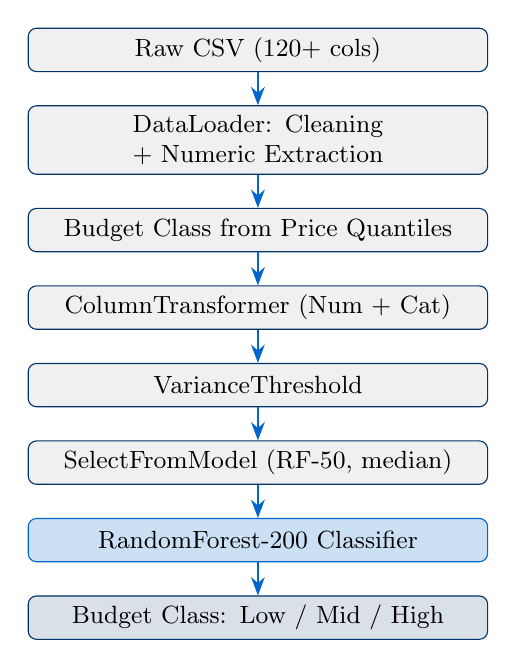
\begin{tikzpicture}[
        node distance=0.42cm,
        box/.style={rectangle, rounded corners=3pt, draw=sctceblue,
                    fill=lightgray, text width=5.6cm,
                    minimum height=0.55cm, align=center, font=\small},
        arrow/.style={-Stealth, thick, color=accentblue}
      ]
        \node[box] (csv)  {Raw CSV (120+ cols)};
        \node[box, below=of csv]  (dl)   {DataLoader: Cleaning + Numeric Extraction};
        \node[box, below=of dl]   (bins) {Budget Class from Price Quantiles};
        \node[box, below=of bins] (ct)   {ColumnTransformer (Num + Cat)};
        \node[box, below=of ct]   (vt)   {VarianceThreshold};
        \node[box, below=of vt]   (sfm)  {SelectFromModel (RF-50, median)};
        \node[box, below=of sfm, fill=accentblue!20, draw=accentblue]
              (rf)   {RandomForest-200 Classifier};
        \node[box, below=of rf, fill=sctceblue!15, draw=sctceblue]
              (out)  {Budget Class: Low / Mid / High};
        \draw[arrow] (csv) -- (dl);
        \draw[arrow] (dl)  -- (bins);
        \draw[arrow] (bins) -- (ct);
        \draw[arrow] (ct)  -- (vt);
        \draw[arrow] (vt)  -- (sfm);
        \draw[arrow] (sfm) -- (rf);
        \draw[arrow] (rf)  -- (out);
      \end{tikzpicture}
  \end{columns}
\end{frame}

% ============================================================
\section{Methodology}
% ============================================================
\begin{frame}{Methodology}
  \begin{itemize}
    \setlength\itemsep{0.45em}
    \item \textbf{Data Cleaning:} Regex extraction \texttt{r"(\textbackslash d+\textbackslash.?\textbackslash d*)"} converts mixed-unit strings
          such as \texttt{"1197 cc"} into numeric values; currency fields are stripped of \texttt{"Rs."}
          and commas before conversion.
    \item \textbf{Critical Rows:} Rows missing \texttt{Ex-Showroom\_Price}, \texttt{Displacement},
          \texttt{Power}, or derived \texttt{Mileage} are removed.
    \item \textbf{Mileage Fallback:} If mileage is missing, it is estimated as
          \[
            \text{Mileage} = \text{clip}\!\left(25 - \frac{CC}{200},\; 5,\; 25\right)
          \]
    \item \textbf{Stage 1 -- Classification:} Random Forest predicts \textbf{Low/Mid/High}
          budget class; CART is retained as an interpretable comparison model.
    \item \textbf{Stage 2 -- Recommendation Ranking:} Candidate cars are ranked using
          similarity between user preference vectors and vehicle specification vectors.
    \item \textbf{Important Separation:} Classification accuracy measures budget prediction;
          match score measures recommendation fit. They are reported separately.
  \end{itemize}
\end{frame}

\begin{frame}{Methodology -- Leakage-Safe Evaluation}
  \begin{columns}[t]
    \column{0.48\textwidth}
      \begin{block}{Correct Evaluation Flow}
        \begin{enumerate}
          \item Load and clean raw vehicle data
          \item Split into train and test sets
          \item Learn budget cutoffs from \textbf{training prices only}
          \item Apply the same cutoffs to the test set
          \item Fit RF/CART only on \texttt{X\_train, y\_train}
          \item Report accuracy only on \texttt{X\_test, y\_test}
        \end{enumerate}
      \end{block}
    \column{0.48\textwidth}
      \begin{alertblock}{Leakage Guards}
        \begin{itemize}
          \item \texttt{Ex-Showroom\_Price} is never used as a feature
          \item \texttt{Budget\_Class} is removed from \texttt{X}
          \item \texttt{Predicted\_Budget\_Class} is dropped before training
          \item \texttt{Similarity\_Score} is dropped before training
          \item Guard tested in \texttt{src/test\_leakage.py}
        \end{itemize}
      \end{alertblock}
  \end{columns}
  \vspace{0.4em}
  \small\textbf{Key point:} Full-data fitting is used only for the final app recommendation flow, not for reporting test accuracy.
\end{frame}

\begin{frame}{Methodology -- Lifestyle Mapping Detail}
  \begin{columns}[t]
    \column{0.51\textwidth}
      \begin{block}{Usage $\rightarrow$ Mileage \& Power}
        \vspace{0.4em}
        \begin{tabular}{lcc}
          \toprule
          \textbf{Usage Pattern} & \textbf{Mileage} & \textbf{Power} \\
          \midrule
          City Commute           & 18 kmpl & 70 BHP  \\
          Highway/Long Distance  & 15 kmpl & 100 BHP \\
          Off-roading            & 10 kmpl & 120 BHP \\
          Family Trips           & 14 kmpl & 90 BHP  \\
          \bottomrule
        \end{tabular}
      \end{block}
      \vspace{0.5em}
      \begin{block}{Passengers $\rightarrow$ Seating}
        $\geq5$ passengers $\Rightarrow$ 7 seats, prefer SUV
      \end{block}

    \column{0.46\textwidth}
      \begin{block}{Experience $\rightarrow$ Power Cap}
        First-time Buyer $\Rightarrow$ Power capped at \textbf{90 BHP}
      \end{block}
      \vspace{0.5em}
      \begin{block}{Priority Weight Adjustment}
        \begin{itemize}
          \item \textit{Fuel Efficiency} prioritizes mileage
          \item \textit{Performance} prioritizes power and lifestyle fit
          \item \textit{Safety} balances mileage, lifestyle, and fuel fit
        \end{itemize}
      \end{block}
      \vspace{0.5em}
  \end{columns}
\end{frame}

% ============================================================
\section{System Workflow}
% ============================================================
\begin{frame}{End-to-End System Workflow}
  \centering
  \includegraphics[height=0.78\textheight,width=0.95\textwidth,keepaspectratio]{workflow.jpg}
\end{frame}

% ============================================================
\section{Model Training \& Testing Cycle}
% ============================================================
\begin{frame}{Model Training \& Testing Cycle}
  \begin{columns}[t]
    \column{0.49\textwidth}
      \textbf{Evaluation Flow}
      \vspace{0.4em}
      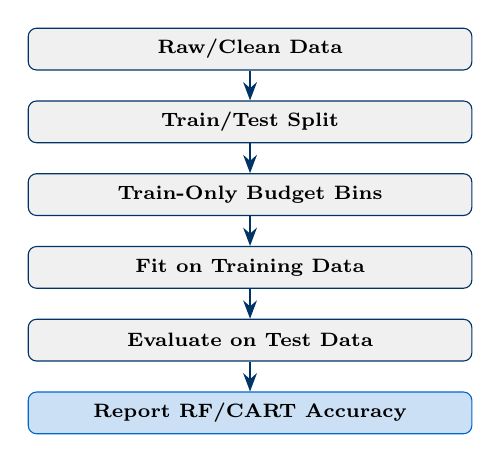
\begin{tikzpicture}[
        node distance=0.38cm,
        box/.style={rectangle, rounded corners=3pt, draw=sctceblue,
                    fill=lightgray, text width=5.4cm,
                    minimum height=0.53cm, align=center, font=\scriptsize\bfseries},
        arrow/.style={-Stealth, thick, color=sctceblue}
      ]
        \node[box] (raw) {Raw/Clean Data};
        \node[box, below=of raw] (split) {Train/Test Split};
        \node[box, below=of split] (bins) {Train-Only Budget Bins};
        \node[box, below=of bins] (fit) {Fit on Training Data};
        \node[box, below=of fit] (test) {Evaluate on Test Data};
        \node[box, below=of test, fill=accentblue!20, draw=accentblue] (score) {Report RF/CART Accuracy};
        \draw[arrow] (raw) -- (split);
        \draw[arrow] (split) -- (bins);
        \draw[arrow] (bins) -- (fit);
        \draw[arrow] (fit) -- (test);
        \draw[arrow] (test) -- (score);
      \end{tikzpicture}

    \column{0.49\textwidth}
      \textbf{Application Flow}
      \vspace{0.4em}
      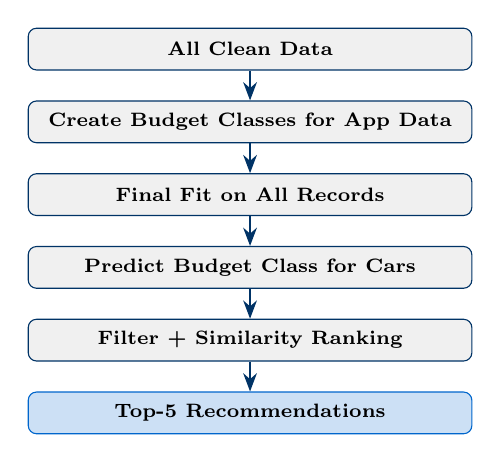
\begin{tikzpicture}[
        node distance=0.38cm,
        box/.style={rectangle, rounded corners=3pt, draw=sctceblue,
                    fill=lightgray, text width=5.4cm,
                    minimum height=0.53cm, align=center, font=\scriptsize\bfseries},
        arrow/.style={-Stealth, thick, color=sctceblue}
      ]
        \node[box] (raw2) {All Clean Data};
        \node[box, below=of raw2] (bins2) {Create Budget Classes for App Data};
        \node[box, below=of bins2] (fit2) {Final Fit on All Records};
        \node[box, below=of fit2] (pred) {Predict Budget Class for Cars};
        \node[box, below=of pred] (rank) {Filter + Similarity Ranking};
        \node[box, below=of rank, fill=accentblue!20, draw=accentblue] (top5) {Top-5 Recommendations};
        \draw[arrow] (raw2) -- (bins2);
        \draw[arrow] (bins2) -- (fit2);
        \draw[arrow] (fit2) -- (pred);
        \draw[arrow] (pred) -- (rank);
        \draw[arrow] (rank) -- (top5);
      \end{tikzpicture}
  \end{columns}
\end{frame}

% ============================================================
\section{Technology Stack}
% ============================================================
\begin{frame}{Technology Stack}
  \begin{center}
    \renewcommand{\arraystretch}{0.75}
    \begin{tabularx}{1.5\textwidth}{>{\bfseries}lX}
      \toprule
      \textbf{Component}      & \textbf{Technology / Library} \\
      \midrule
      Language                & Python 3.x \\
      UI Framework            & Streamlit \\
      Data Handling           & Pandas, NumPy \\
      Data Cleaning           & Pandas regex, \texttt{str.extract}, \texttt{pd.to\_numeric} \\
      Preprocessing           & Scikit-Learn \texttt{ColumnTransformer}, \texttt{MinMaxScaler}, \texttt{SimpleImputer} \\
      Feature Reduction       & Scikit-Learn \texttt{VarianceThreshold}, \texttt{SelectFromModel} \\
      Classification          & \texttt{RandomForestClassifier}, \texttt{DecisionTreeClassifier} \\
      Evaluation              & \texttt{train\_test\_split}, \texttt{StratifiedKFold}, confusion matrix, classification report, dummy baseline \\
      Ranking                 & Scikit-Learn \texttt{cosine\_similarity} / weighted similarity score \\
      Model Persistence       & \texttt{joblib} for saved Random Forest and CART pipelines \\
      \bottomrule
    \end{tabularx}
  \end{center}
  \vspace{0.3em}
  \small\textbf{Key Dependencies from \texttt{requirements.txt}:}
  \texttt{joblib==1.5.3} \quad \texttt{scikit-learn==1.8.0} \quad \texttt{pandas==3.0.0} \quad
  \texttt{numpy==2.4.2} \quad \texttt{scipy==1.17.0}
\end{frame}

% ============================================================
\section{Results}
% ============================================================
\begin{frame}{Results -- Clean Evaluation}
  \begin{columns}[t]
    \column{0.46\textwidth}
      \begin{block}{Holdout Evaluation}
        \vspace{0.3em}
        \begin{tabular}{lc}
          \toprule
          \textbf{Metric} & \textbf{Score} \\
          \midrule
          Dummy Baseline & 36.36\% \\
          CART Decision Tree & 88.11\% \\
          Random Forest & \textbf{90.91\%} \\
          \bottomrule
        \end{tabular}
      \end{block}
      \vspace{0.5em}
      \begin{block}{Cross-Validation}
        \vspace{0.3em}
        \begin{tabular}{lc}
          \toprule
          \textbf{Method} & \textbf{RF Accuracy} \\
          \midrule
          Stratified 5-Fold CV & \textbf{92.54\%} \\
          Variation & $\pm$4.25\% \\
          \bottomrule
        \end{tabular}
      \end{block}

    \column{0.51\textwidth}
      \begin{block}{Top RF Feature Importances}
        \vspace{0.3em}
        \begin{tabular}{lc}
          \toprule
          \textbf{Feature} & \textbf{Importance} \\
          \midrule
          Power & 0.1030 \\
          Displacement & 0.0626 \\
          Wheelbase & 0.0601 \\
          Seat Height Adjustment & 0.0587 \\
          Torque & 0.0511 \\
          Length & 0.0455 \\
          Number of Airbags & 0.0447 \\
          Kerb Weight & 0.0388 \\
          Width & 0.0378 \\
          \bottomrule
        \end{tabular}
      \end{block}
      \vspace{0.4em}
  \end{columns}
\end{frame}

\begin{frame}{CART Model Explainability}
  \centering
  \includegraphics[width=0.96\textwidth,height=0.78\textheight,keepaspectratio]{cart.jpg}
  \vspace{0.2em}

  \small CART is used as an interpretable comparison model for budget class prediction;
  Random Forest remains the primary classifier.
\end{frame}

% ============================================================
\section{Conclusion}
% ============================================================
\begin{frame}{Conclusion}
  \begin{itemize}
    \setlength\itemsep{0.1em}
    \item \textbf{AutoMatch} demonstrates that a two-stage ML pipeline can solve vehicle
          recommendation by first classifying budget tier and then ranking suitable cars.
    \item Random Forest provides strong budget prediction performance, while CART supports
          interpretability and comparison.
    \item The recommendation score is used only for ranking user-fit, keeping it separate
          from classification accuracy.
  \end{itemize}
  \vspace{0.3em}
  \begin{block}{Future Scope}
    \begin{columns}[t]
      \column{0.48\textwidth}
        \begin{itemize}
          \item Real-time dealer pricing and availability APIs
          \item Saved model deployment with scheduled refresh
        \end{itemize}
      \column{0.48\textwidth}
        \begin{itemize}
          \item User feedback loop for preference refinement
          \item EV-specific recommendation with range and charging features
        \end{itemize}
    \end{columns}
  \end{block}
\end{frame}

% ============================================================
\section{References}
% ============================================================
\begin{frame}{References}
  \footnotesize
  \begin{thebibliography}{9}
    \bibitem{ricci2025}
      F.\ Ricci \textit{et al.}
      ``Responsive Web-Based Car Recommendation System With AI-Based Filtering.''
      \textit{IEEE International Conference on Artificial Intelligence},
      pp.\ 112--118, 2025.

    \bibitem{prabowo2022}
      G.\ Prabowo \textit{et al.}
      ``Machine Learning-Powered Car Recommendation System: A Content-Based Approach.''
      \textit{International Research Journal of Engineering and Technology (IRJET)},
      Vol.\ 9, No.\ 10, pp.\ 153--159, 2022.

    \bibitem{senanayake2020}
      J.\ Senanayake \textit{et al.}
      ``Vehicle Recommendation System using Hybrid Recommender Algorithm.''
      \textit{2nd International Conference on Advancements in Computing (ICAC)},
      IEEE, pp.\ 240--245, 2020.

    \bibitem{sklearn2011}
      F.\ Pedregosa \textit{et al.}
      ``Scikit-learn: Machine Learning in Python.''
      \textit{Journal of Machine Learning Research},
      Vol.\ 12, pp.\ 2825--2830, 2011.

    \bibitem{mckinney2010}
      W.\ McKinney.
      ``Data Structures for Statistical Computing in Python.''
      \textit{Proceedings of the 9th Python in Science Conference},
      pp.\ 51--56, 2010.

    \bibitem{cardekho}
      CarDekho.
      \textit{Indian Passenger Vehicle Listings Dataset}.
      Available at: \texttt{https://www.cardekho.com}, Accessed April 2026.

    \bibitem{streamlit}
      Streamlit Inc.
      \textit{Streamlit Documentation}.
      Available at: \texttt{https://docs.streamlit.io}, Accessed April 2026.
  \end{thebibliography}
\end{frame}

% ---------- Thank You ----------
\begin{frame}
  \centering
  \vspace{2em}
  {\Huge\color{sctceblue}\textbf{Thank You}}\\[1em]
  {\large Questions \& Feedback Welcome}\\[2em]
  \begin{columns}[c]
    \column{0.33\textwidth}\centering \textbf{Aadil Sandeep}\\\small Roll No.\ 301
    \column{0.33\textwidth}\centering \textbf{Adithyan R}\\\small Roll No.\ 305
    \column{0.33\textwidth}\centering \textbf{Adhway Satheesh}\\\small Roll No.\ 366
  \end{columns}
  \vspace{1em}
  \small Guided by \textbf{Dr.\ Rejimoan R} $\cdot$ SCTCE, Thiruvananthapuram
\end{frame}

\end{document}
